\subsection{Протокол Station-to-Station}\label{section-protocols-sts}\index{протокол!Station-to-Station|(}
\selectlanguage{russian}

Протокол STS (\langen{Station-to-Station},~\cite{Diffie:Oorschot:Wiener:1992})\index{протокол!Station-to-Station} предназначен для систем мобильной связи. Он использует идеи протокола Диффи~---~Хеллмана\index{протокол!Диффи~---~Хеллмана} и криптосистемы RSA\index{криптосистема!RSA}. Особенностью протокола является использование механизма электронной подписи\index{электронная подпись} для взаимной аутентификации сторон\index{аутентификация!взаимная}.

Предварительно стороны договорились об общих параметрах системы $p$ и $g$, где $p$ -- большое простое число, а $g$ -- примитивный элемент поля $\Z_p^*$.

Каждая из сторон $A$ и $B$ обладает долговременной парой ключей: закрытым ключом для расшифрования и создания электронной подписи $K_{\text{public}}$ и открытым ключом для шифрования и проверки подписи $K_{\text{public}}$.

\[\begin{array}{ll}
    A: K_{A,\text{private}}, K_{A,\text{public}}: \forall M : & \text{Verify}_A ( M, S_A( M ) ) = true, \\
                                                & D_A ( E_A( M ) ) = M, \\
    B: K_{B,\text{private}}, K_{B,\text{public}}: \forall M : & \text{Verify}_B ( M, S_B( M ) ) = true, \\
                                                & D_B ( E_B( M ) ) = M. \\
\end{array}\]

Где $\text{Verify}_A(\dots)$ это функция проверки электронной подписи на открытом ключе $K_{A, \text{public}}$, а $D_A$ -- функция расшифрования с использованием закрытого ключа $K_{A, \text{private}}$.

Протокол состоит из четырёх проходов, три из которых включают передачу сообщений (рис.~\ref{fig:key_distribution-sts}, \cite{Cheremushkin:2009}).

\begin{figure}
    \centering
    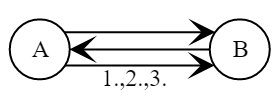
\includegraphics[width=0.5\textwidth]{pic/key_distribution-sts}
    \caption{Взаимодействие участников в протоколе STS\label{fig:key_distribution-sts}}
\end{figure}

\begin{protocol}
    \item[(1)] Алиса выбирает случайное число $R_A: 2 \leq R_A \leq p-1$.
    \item[{}] $Alice \to \left\{ A, m_A = g^{R_A} \bmod p \right\} \to Bob$

    \item[(2)] Боб выбирает случайное число $R_B: 2 \leq R_B \leq p-1$.
    \item[{}] Боб вычисляет сессионный ключ $K = m_A^{R_B} \bmod p$.
    \item[{}] $Bob \to \left\{ B, A, m_B = g^{R_B} \bmod p, E_K( S_B ( m_A, m_B )) \right\} \to Alice$

    \item[(3)] Алиса вычисляет сессионный ключ $K = m_B^{R_A} \bmod p$.
    \item[{}] Алиса проверяет подпись в сообщении $E_K( S_B ( m_A, m_B ))$.
    \item[{}] $Alice \to \left\{ A, B, E_K( S_A ( m_A, m_B ) ) \right\} \to Bob$

    \item[(4)] Боб проверяет подпись в сообщении $E_K( S_A ( m_A, m_B ))$.
\end{protocol}

Протокол обеспечивает арантию формирования новых ключей (G10), но не совершенную прямую секретность (G9).

Как показала атака Лоу 1996 года (\cite{Lowe:1996}, рис.~\ref{fig:key_distribution-sts-attack}), протокол не может гарантировать аутентификацию субъектов (цель G1), ключей (G7) и подтверждение владения сессионным ключом (G8). Хотя злоумышленник не может получить доступ к новому сессионному ключу, если протокол использовать только для аутентификации субъектов, Алиса может принять злоумышленника за Боба.

\begin{figure}
    \centering
    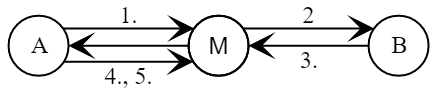
\includegraphics[width=0.67\textwidth]{pic/key_distribution-sts-attack}
    \caption{Схема взаимодействия участников в протоколе STS при атаке Лоу\label{fig:key_distribution-sts-attack}}
\end{figure}

\begin{protocol}
    \item[(1)] Алиса выбирает случайное число $R_A: 2 \leq R_A \leq p-1$.
    \item[{}] $Alice \to \left\{ A, m_A = g^{R_A} \bmod p \right\} \to Mellory~(Bob)$

    \item[(2)] $Mellory \to \left\{ M, m_A \right\} \to Bob$

    \item[(3)] Боб выбирает случайное число $R_B: 2 \leq R_B \leq p-1$.
    \item[{}] Боб вычисляет сессионный ключ $K = m_A^{R_B} \bmod p$.
    \item[{}] $Bob \to \left\{ B, M, m_B, E_K( S_B ( m_A, m_B )) \right\} \to Mellory$

    \item[(4)] $Mellory~(Bob) \to \left\{ B, A, E_K( S_B ( m_A, m_B )) \right\} \to Alice$

    \item[(5)] Алиса вычисляет сессионный ключ $K = m_B^{R_A} \bmod p$.
    \item[{}] Алиса проверяет подпись в сообщении $E_K( S_B ( m_A, m_B ))$.
    \item[{}] $Alice \to \left\{ A, B, E_K( S_A ( m_A, m_B ) ) \right\} \to Mellory~(Bob)$
\end{protocol}

После успешного завершения протокола Алиса уверена, что общается с Меллори.

Как и все остальные <<криптосистемы-протоколы>>, протокол Station-to-Station основывается на некотором внешнем источнике информации об открытых ключах участников, не подвергая сомнению корректность и надёжность этого источника. Что, в общем случае, неверно. Если информация о ключах участников нужно получать извне при каждом сеансе протокола (например, если участников много, и запомнить ключи всех возможности нет), то канал получения открытых ключей будет основной целью активного криптоаналитика для рассмотренных протоколов. Как от этого защититься с использованием примитивов асимметричной криптографии -- в следующем разделе.

\index{протокол!Station-to-Station|)}